\section{Introduction}%
\label{sec:intro_PO}

\subsection{Quelle métrique pour l'impact sanitaire ?}%
\label{sub:quelle_métrique_pour_l_impact_sanitaire_}


Bien que dans les chapitres précédents nous avons vu qu'il était possible d'estimer de
façon fiable la contribution des différentes sources de PM grâce à la méthodologie PMF et d'établir une
phénoménologie des sources de \PMdix, la question de leurs effets sanitaires respectifs est toujours sans réponse. En effet, l'ordre de contribution à la concentration moyenne annuelle des
\PMdix{} présentée par \cite[(figure 3)]{weberComparison2019} ne préjuge pas de leurs
impacts sanitaires.

En effet, comme détaillé en introduction
section~\ref{sec:le_potentiel_oxydant_des_aerosols}, la mesure de la masse des PM n'est
certainement pas l'indicateur le plus adapté pour évaluer leur toxicité, car les propriétés
physico-chimiques qui la détermine (la composition
chimique, forme, surface réactive, etc.) ne sont pas prises en compte par cette métrique.
C'est pourquoi le potentiel oxydant (PO ou OP en anglais), mesurant indirectement les
espèces réactives de l'oxygène (ERO ou ROS en anglais) apportées ou générées par les PM,
est proposé comme nouvel indicateur de l'exposition des populations à la pollution particulaire. 
Il est maintenant bien documenté que les différents tests de PO présentent une information
différente de la concentration massique (voir par exemple,
\cite{choRedox2005,vermaReactive2014,batesReactive2015,fangOxidative2016,fangAmbient2017,calasSeasonal2019},
ou la revue détaillée récente de \cite{batesReview2019}).
% , comme rappelé dans le
% tableau~\ref{tab:calas_2018_spearman} sur une étude à Chamonix par
% \cite{calasComparison2018} présentant la corrélation entre la masse des \PMdix{} et 5
% mesures de PO.


À titre d'exemple, les moyennes des concentrations massiques et de \POAAv{} pour 4 sites (Bolivie,
Inde, Suisse et France) analysés à l'IGE sont présentées figure~\ref{fig:OPAAv_4sites}.
Alors que la concentration massique est identique pour chacun des couples
Cochambamba-Dehli et Strasbourg-Berne, le \POAAv{} varie d'un facteur 2 à 3.  Ainsi, si
le site de Berne présente des concentrations en \PMdix{} inférieur au seuil réglementaire
et 5 fois plus faible que le site urbain de Cochabamba, le \POAAv{} de ces \PMdix{} est
en réalité 2 fois supérieure, indiquant en définitive des \PMdix{} ayants une activité
oxydante beaucoup plus importante sur le site de Berne que de Cochabamba, et donc
probablement un impact sanitaire plus délétère alors que la métrique de la masse seule
donnerait la conclusion inverse.
Cependant, il existe aussi de lieux de prélèvement où les 2 métriques concordent. Sur le
site de Dehli, à la fois la masse et le \POAAv{} des \PMdix{} sont élevées, et sur le
site de Strasbourg, de faible concentration massique sont associés à de faible \POAAv.

La mise en regard de ces deux métriques, apporte une vision différente de l'exposition
aux particules.
En ne mesurant qu'une quantité, la concentration massique des PM ne capture pas la complexité
des propriétés physico-chimiques de l'aérosol en présence. Si on postule que le PO est
un meilleur indicateur de l'impact sanitaire des PM car il intègre un plus grand 
nombre des propriétés qui font la toxicité des particules, alors, cet exemple illustre
que la masse est peu adaptée à l'étude de la qualité de l'air concertant l'exposition 
des populations.


\begin{figure}[ht!]
    \centering
    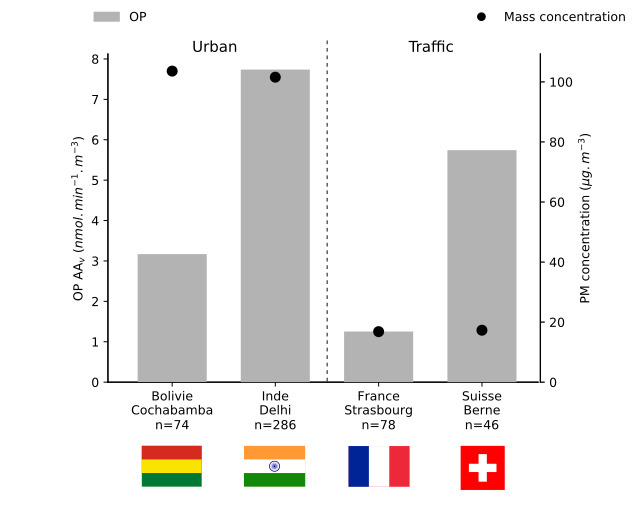
\includegraphics[width=0.7\linewidth]{figures/chapter04/OPAAv_4sites.png}
    \caption{Comparaison de la métrique de la masse et du \POAAv{} des PM, pour 2 pairs
        de sites urbain et trafic présentant une même concentration massique de PM
        moyenne identique mais des \POAAv{} très différents. Mesures effectuées à l'IGE.\\
        Crédit: PSI pour le site de Berne, X pour Dehli, programme interne pour
        Cochambamba et Strasbourg.
    }%
    \label{fig:OPAAv_4sites}
\end{figure}


% \begin{table}[ht]
%     \begin{ThreePartTable}
%         \centering
%         \caption{Corrélation de Spearman entre 5 tests de PO et la masse des \PMdix{} sur
%             le site de Chamonix (2013) séparer en période chaude (triangle bas) et froide
%             (triangle haut).\\
%             Source : \cite[Table 3]{calasComparison2018}
%         }
%         \label{tab:calas_2018_spearman}
%         \footnotesize
%         \begin{tabular}{lSSSSSS}
%             \toprule
%              & {\PMdix} & {OP DTTv\tnote{1}} & {OP AAv\tnote{1}} & {OP ESRv\tnote{2}} & {OP GSHv\tnote{1}} & {OP ASCv\tnote{3}}\\
%              \midrule
%             \PMdix  &           & 0.91{***} & 0.91{***} & 0.59{***} & 0.87{***} & 0.90{***}\\
%             OP DTTv & 0.71{***} &           & 0.89{***} & 0.61{***} & 0.79{***} & 0.72{***}\\
%             OP AAv  & 0.43{*}   & 0.65{***} &           & 0.54{***} & 0.85{***} & 0.79{***}\\
%             OP ESRv & 0.088     & 0.17      & 0.36      &           & 0.56{**}  & 0.59{**}\\
%             OP GSHv & 0.44{*}   & 0.29      & 0.36      & 0.63{*}   &           & 0.92{***}\\
%             OP ASCv & 0.38{*}   & 0.37{*}   & -0.072    & -0.29     & 0.17      & \\
%             \bottomrule
%         \end{tabular}
%         \begin{tablenotes}
%         \item[] *** p < 0.001 level, ** p < 0.01 level, * p < 0.05 level
%         \item[1] n = 30 (cold period), n = 29 (warm period)
%         \item[2] n = 30 (cold period), n = 14 (warm period)
%         \item[3] n = 27 (cold period), n = 29 (warm period)
%         \end{tablenotes}
%     \end{ThreePartTable}
% \end{table}

\subsection{Un PO par espèces chimiques ?}%
\label{sub:un_po_par_espèces_chimiques_}

Il est également connu que les différentes espèces chimiques constitutives des PM ne
réagissent pas à un même test de PO de la même manière. Notamment, les métaux de
transitions ainsi que certaines quinones conduisent à la formation d'un grand nombre de
\ce{HO^.} et sont donc des espèces très réactives à la mesure du PO
\autocite{charrierRates2015,calasImportance2017}.

Cependant, lorsque l'ensemble des PM est solubilisé, analysé et confronté aux différents tests de PO, de
fortes corrélations sont bien observées avec les espèces présentant une forte réactivité aux
PO, mais certaines autres espèces sont parfois fortement corrélées alors que la mesure directe de leur PO est nulle (tous tests confondus) --c'est notamment le cas du nitrate,
de l'ammonium, du lévoglucosan ou du \ce{Fe^{II}}~\autocite{vermaRedox2009,calasComparison2018,calasSeasonal2019}.

Ces corrélations ne reflètent donc pas nécessairement de réelles causalité mais des
co-corrélations. Le lévoglucosan est émis en même temps que certaines quinones lors de la
combustion de bois, qui elles sont redox-actives, et le nitrate est émis de façon saisonnière en
fin de l'hiver alors que la combustion de biomasse est toujours présente.  Ainsi, ces
corrélations sont un premier pas vers l'identification des sources majoritaires de PO,
mais s'avère insuffisantes.

\subsection{Du PO par espèce chimique au PO par source}

L'attribution d'un PO intrinsèque par espèce chimique est donc estimée par mesure
directe ou par régression linéaire
multiple~\autocite{calasImportance2017,borlazaOxidative2018}. La première solution permet
la mesure exacte du PO de l'espèce mais présente des limitations analytiques évidentes
(composé pur, grand nombre d'espèces et de gamme de concentration à étudier), et la
deuxième peut présenter des ``faux positifs'' dans le cas où toutes les espèces chimiques
ne sont pas mesurées --ce qui est toujours le cas-- du fait de l'émission conjointe
d'espèces redox-actives et non-redox-actives (quinones et lévoglucosan par exemple).

Aussi, d'un point de vue réglementaire, il est souvent plus compréhensible d'agir sur
un secteur d'émission que sur une espèce chimique en particulier.

Pour ces raisons, l'agrégation de l'information géochimique par source d'émission plutôt
que par espèce chimique est intéressante :
\begin{enumerate}
    \item le nombre d'inconnues diminue drastiquement (plusieurs milliers d'espèces
        chimique à une dizaine de sources d'émission);
    \item le besoin d'identifier chaque espèce chimique disparaît si les sources
        majoritaires sont bien représentées;
    \item la contribution des sources au potentiel oxydant est davantage transmissible
        en termes de politiques publiques que la contribution d'espèces chimiques;
\end{enumerate}

Pour estimer un PO par source, plusieurs méthodes sont possibles : 1) introduire le PO
comme variable dans une étude de source (CMB, PMF, etc.) 2) faire une étude de source
(CMB, PMF, etc.) grâce à l'information chimique et ensuite établir un modèle d'inversion
entre les sources identifiées et les différentes mesures de PO.

\cite{vermaReactive2014} ont utilisé les 2 méthodes en introduisant le
\PODTT{} dans une PMF avec comme autres espèces WSOC\footnote{WSOC: Water soluble
organic carbon}, BrnC\footnote{BrnC: Brown Carbon}, EC, \SOq, \NHt, K, Ca, Mn, Fe, Cu et
Zn, mais également en établissant une régression linéaire entre le \PODTT{} et les sources
issues du CMB.
Entre 2014 et 2017, \cite{batesReactive2015} puis \cite{fangOxidative2016}, de la même
équipe de recherche, ont repris ce principe et l'ont appliqué à plus grande échelle
spatiale et également au \POAAv.\footnote{Lors du commencement de ma thèse, à ma connaissance, seules ces 3 études étaient
disponibles dans la littérature. Ce sujet s'est vu largement développé au cours des 3
dernières années, et sera discuté dans la suite.}

\begin{figure}[ht]
    \centering
    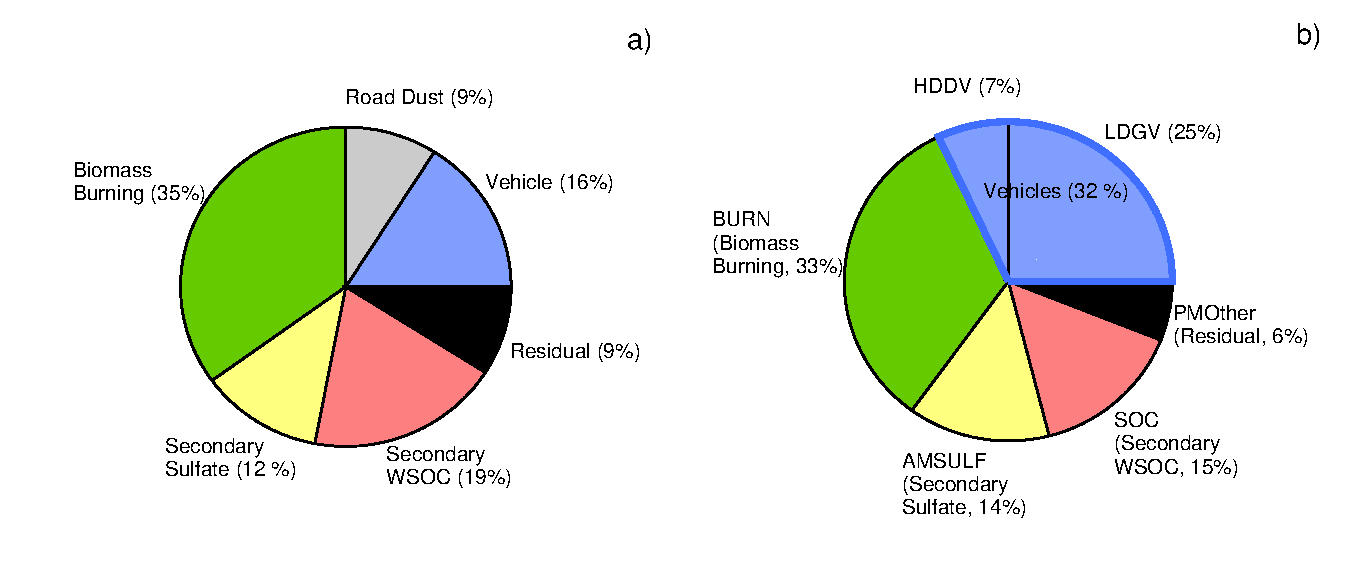
\includegraphics[width=1.0\linewidth]{figures/chapter04/verma_2014_fig8.pdf}
    \caption{Première estimation de la contribution des sources de PM au \PODTT{} par
        \cite[][figure 8]{vermaReactive2014}: \textbf{a)} par ajout du DTT dans la PMF et
        \textbf{b)} par régression linéaire entre \PODTT{} et CMB.
    }%
    \label{fig:figures/chapter04/verma_2014_fig8}
\end{figure}

Seulement, nous avons vu que les études de sources utilisant la méthodologie PMF sont très sensibles aux variables utilisées. Or, les
études PMF précédemment citées incluent un ensemble d'espèces chimiques restreint (une dizaine de métaux et le
WSOC), en plus du PO. Seuls 4 facteurs sont identifiés par~\cite{fangOxidative2016}, ce
qui semble peu au regard des études PMF utilisant un jeu d'espèces chimiques plus conséquent (cf.
notamment tout le chapitre précédent). De plus, ce faible nombre de composés atmosphériques
associés à une nouvelle variable, le PO, dont la connaissance \textit{a priori} des sources qui l'influence de façon spatio-temporelle reste très limitée , peut conduire à des solutions instables statistiquement.

La solution utilisant la régression linéaire à partir du CMB hérite des limitations
propres au CMB : peu de prise en compte des particularités locales, connaissance a priori
forte, etc (voir section~\ref{ssub:atouts_et_limitations_des_différents_modèles_récepteurs}).
Ainsi, \cite{batesSource2018} utilise un modèle CMB pour prédire à large échelle spatiale
(Amérique du Nord) le PO, mais le modèle établit présent de faibles performances
statistiques ($r^2 = 0.36$ et intercepte non nul), notamment du fait de l'oubli potentiel de
sources importantes (bioaérosols \autocite{samakeUnexpected2017}, etc).

\subsection{Couplage de la méthodologie PMF avancée avec l'estimation du PO}%
\label{sub:couplage_de_pmf_avancée_avec_l_estimation_du_po}

Dans ce chapitre, je propose tout d'abord une méthodologie permettant de coupler les
connaissances acquises sur les études PMF présentées
dans le chapitre~\ref{cha:approfondissement_des_connaissances_des_sources_des_pm}
précédent, en n'ajoutant pas le PO comme variable explicative pour ne pas perturber le
modèle, puis d'évaluer le PO intrinsèque (i.e. par microgramme) de chacune des sources
identifiées, illustré par la figure~\ref{fig:workflow_inversion}.

Le site de Chamonix entre 2013 et 2014 a été choisi pour tester cette méthode du fait
d'une étude PMF approfondie par \cite{chevrierChauffage2016} et par les mesures de PO sur
ce site effectué lors de la thèse de \cite{calasPollution2017}, aussi bien pour le \POAA{}
que le \PODTT, et a fait l'objet d'une publication~\autocite{weberApportionment2018}
présentée dans la section~\ref{sec:weber_et_al_2018}.

Cette méthode ayant présenté des résultats très encourageants, son application à un
ensemble de 15 séries de prélèvements réparties sur 14 sites en France métropolitaine est
discutée dans la section~\ref{sec:synthèse_grande_échelle}.
Cette partie reprend un article en cours de soumission~\autocite{weberSourceinprep.} et a
déjà été présentée à l'EAC de 2019 à Göteburg \autocite{weberSources2019}.

\begin{figure}[ht]
    \centering
    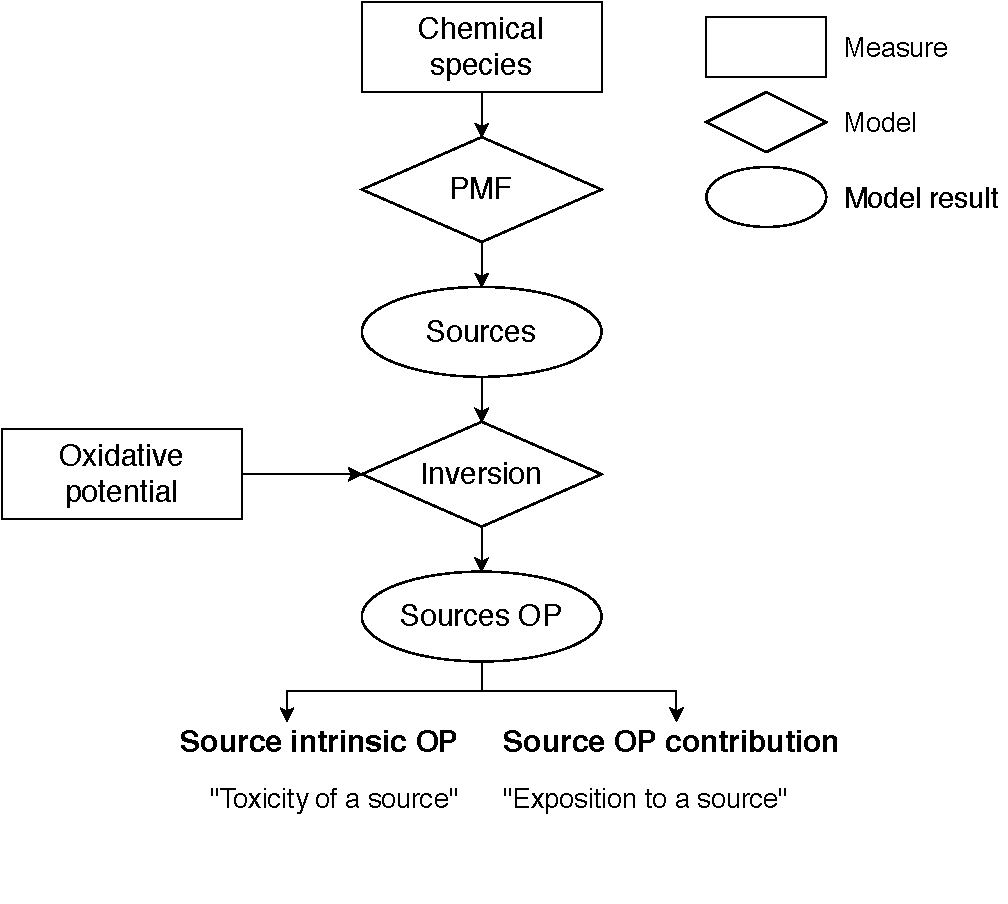
\includegraphics[width=0.8\linewidth]{figures/chapter04/flowchart_inversion.pdf}
    \caption{Processus suivi afin d'estimer la contribution des sources de PM aux
        potentiels oxydants. La méthode d'inversion utilisée dans ce chapitre est une
        régression linéaire multiple, permettant d'attribuer un PO par microgramme de source
        (\textit{PO intrinsèque}), estimant la ``toxicité de la source'', et la contribution de
    chacune des sources aux PO, estimant l'exposition de la population à cette source.}%
    \label{fig:workflow_inversion}
\end{figure}


\section{Généralisation de la mesure du PO}%
\label{sec:généralisation_de_mesure_du_po}

\subsection{Climatologie du PO}%
\label{sub:climatologie_du_po}

\begin{tcolorbox}[colback=red!5!white,colframe=Melon,title=Note]
    Une partie des résultats présentés dans cette section s'appuie sur l'article de
    \cite{calasSeasonal2019}, pour lequel mon implication a porté notamment sur la mise à
    disposition et visualisation des données disponibles à
    \url{https://pmall.univ-grenoble-alpes.fr/OP}.\\
    La généralisation à davantage de sites d'études est également présentée dans cette
    partie.
\end{tcolorbox}

\subsubsection{Variabilité saisonnière}%
\label{ssub:variabilité_saisonnière}

Les mesures de PO effectuées à l'IGE permettent d'établir une climatologie du potentiel
oxydant sur une large échelle spatiale, et pour différents types d'environnement. Cette
base de données unique permet la mise en lumière d'une variation temporelle du \POAAv{} et
\PODTTv{} (voir figure~\ref{fig:variabilite_saisonniere}), comme déjà rapporté dans
différentes études présentant des résultats annuels
\autocite{fangOxidative2016,calasComparison2018,calasSeasonal2019,pietrograndePM102018}.

Cependant, cette variation saisonnière n'est pas observée pour l'ensemble des typologies
de sites. Elle est notamment très marquée sur les sites de vallées alpines mais beaucoup
moins pour les sites de bord de mer et portuaires (voir
figure~\ref{fig:variabilite_saisonniere_MRS_PASSY} pour le site de Passy (vallée alpine)
et Marseille-5 avenues (urbain et marin)).

En définissant la saison chaude sur la période d'avril à septembre et la saison froide
d'octobre à mars, le \POAAv{} présente des contrastes saisonniers beaucoup plus marqués que
le \PODTTv. Dans l'étude de \cite[tableau 3]{calasSeasonal2019}, sur les 7 sites étudiés,
le \POAAv{} est jusqu'à 6 fois plus élevé en hiver qu'en été pour le site de Chamonix
alors que ce ratio n'est que de 2 pour le \PODTTv. De manière générale, l'amplitude des
variations saisonnières du \PODTTv{} est similaire à celle de la masse des \PMdix{} alors
que le \POAAv{} présente des variations beaucoup plus importantes.

En plus d'être une première indication sur les sources d'émission influençant
majoritairement les différents tests de PO, la connaissance de cette variation saisonnière
ou son absence pourrait contraindre de manière plus efficace les extrapolations des
modèles épidémiologiques et de \textit{Land Use Regression} utilisant des extrapolations à
partir de quelques semaines de mesures uniquement
\autocite{yangaileenSpatial2015,jedynskaSpatial2017}.

\begin{figure}[ht]
    \centering
    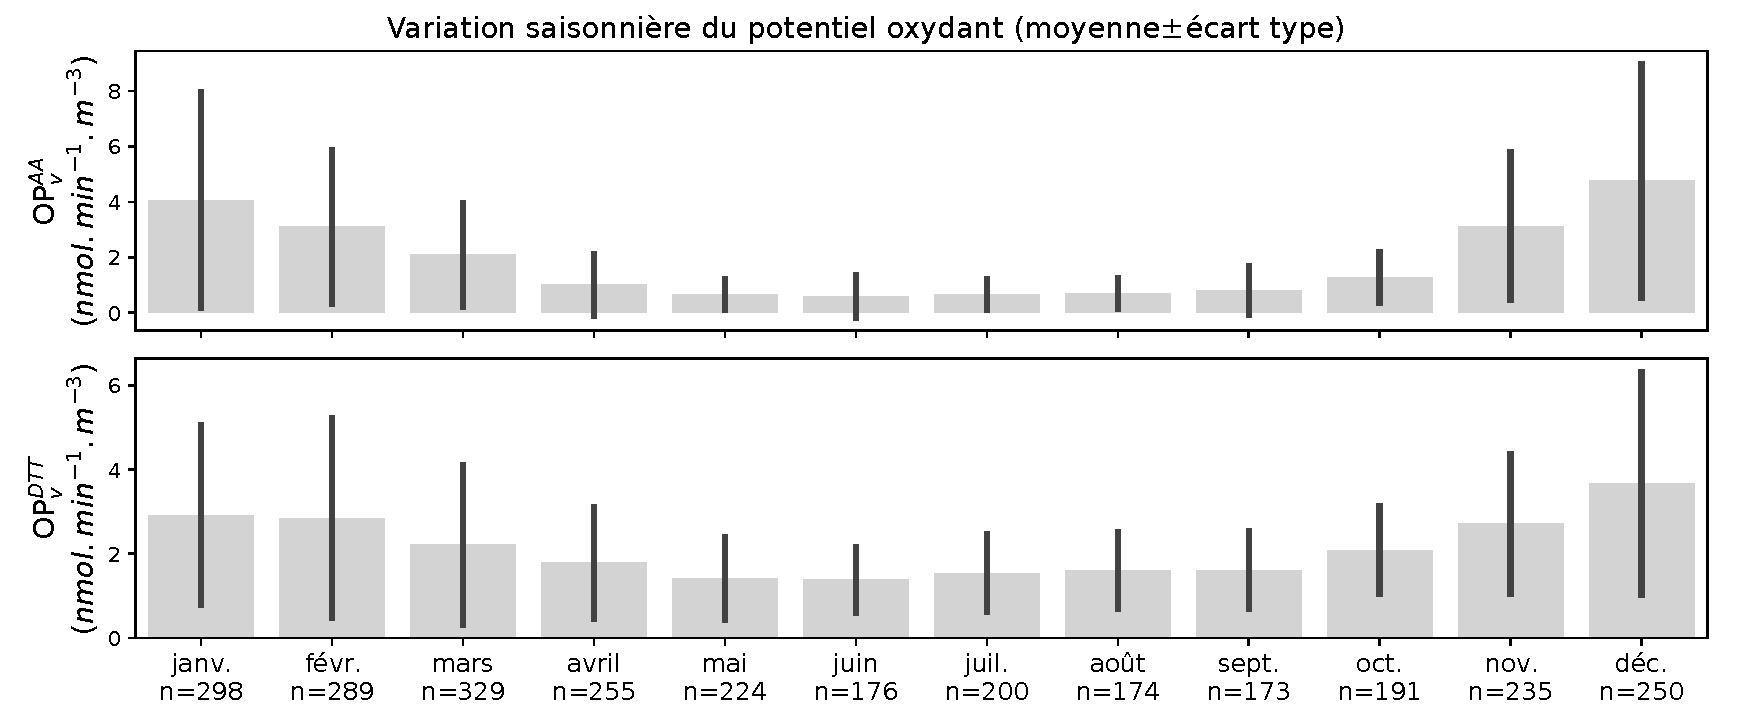
\includegraphics[width=1.0\linewidth]{figures/chapter04/variabilite_saisonniere.pdf}
    \caption{Variabilité saisonière du \POAAv{} et \PODTTv{} sur 16 sites de prélévements
        de \PMdix{} en France métropolotaine pour un total de 3458 échantillons.
    }%
    \label{fig:variabilite_saisonniere}
\end{figure}


\begin{figure}[ht]
    \centering
    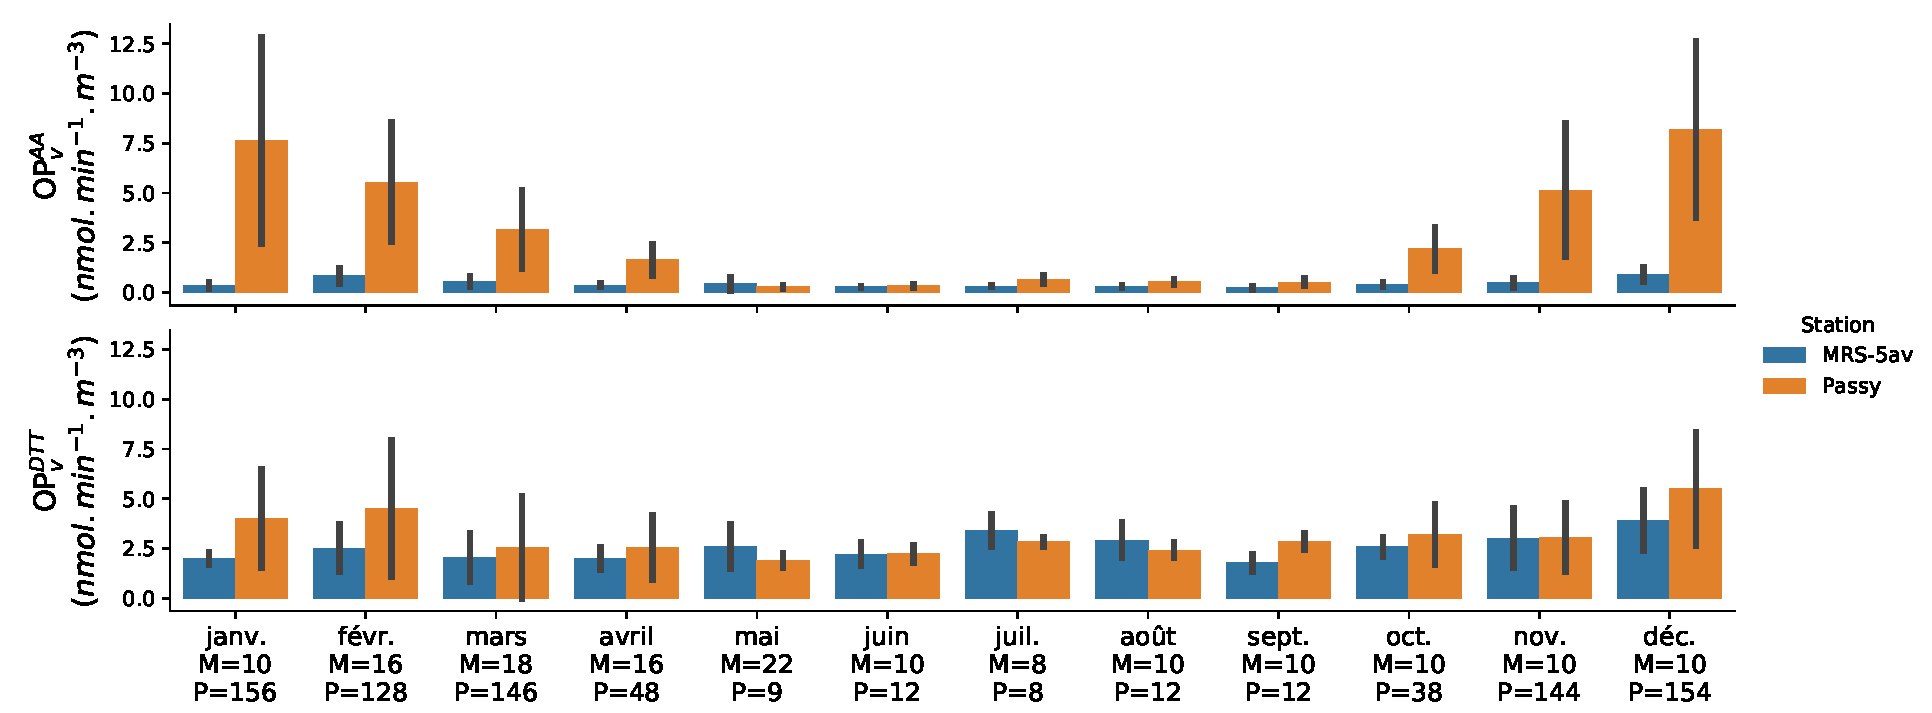
\includegraphics[width=1.0\linewidth]{figures/chapter04/variabilite_saisonniere_MRS-Passy.pdf}
    \caption{Détail de la variabilité saisonière du \POAAv{} et \PODTTv{} sur le site de
        Passy (vallée alpine de l'Arve) en orange et le site urbain et portuaire de MRS-5av
        (Marseille) en bleu.
    }%
    \label{fig:variabilite_saisonniere_MRS_PASSY}
\end{figure}

\subsubsection{Variabilité des corrélations chimie -- PO}%
\label{ssub:_variabilité_des_corrélations_chimie_po}

À cette différenciation des valeurs de \POv{} selon la typologie des sites s'ajoute des
corrélations différentes avec les espèces chimiques, notamment entre le \POAAv{} et le
Cu, Sb et Sn entre les sites de la vallée de l'Arve (Chamonix, Passy et Marnaz) et les
autres sites (Talence, Grenoble, Nice, Port-de-bouc). La figure 7 de
\cite{calasSeasonal2019} illustre cette plus forte corrélation entre le Cu et le \POAAv{}
pour ces 3 sites de la vallée de l'Arve. Cette importance accrue des traceurs des
émissions hors échappement dans la vallée de l'Arve reste peu comprise. Une hypothèse
avancée pourrait être la présence plus importante de camion de transit dans cette vallée
comparée aux autres sites d'études.

Cependant, les tendances des corrélations entre PO et espèces chimiques sont bien
similaires sur l'ensemble des sites. Une généralisation est présentée
figure~\ref{fig:pairplotOPs} pour l'OC, EC, Lévoglucosan, \NOt, Cu et Fe sur un ensemble
de 16 sites de prélèvements en France pour un total de plus de 3400 échantillons.
Conformément aux études antérieures, l'OC, EC et Lévoglucosan sont fortement corrélés
aux différents tests de PO, et de façon très notable au \POAAv. Concernant le nitrate, cuivre et fer en revanche, ces
corrélations sont aussi positives mais semblent dépendre du site considéré.
En revanche, et comme déjà exposé, les corrélations ne sont pas suffisantes pour conclure
à une quelconque association ou causalité, ces co-variations pouvant aussi être imputées à des composés co-émis par la même source de particules. 

\begin{figure}[ht]
    \centering
    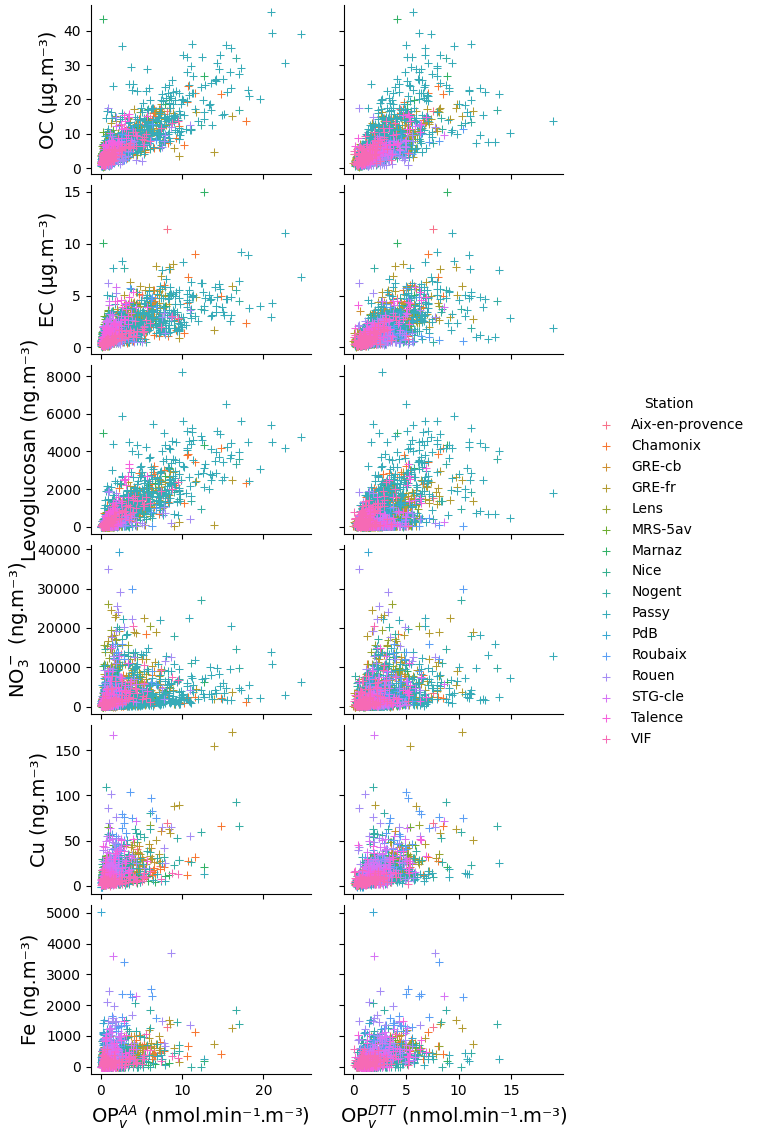
\includegraphics[width=0.7\linewidth]{figures/chapter04/pairplot_OPs.png}
    \caption{Relation entre les \POAAv{} et \PODTTv{} et l'OC, EC, Lévoglucosan, \NOt, Cu et Fe pour
    3458 échantillons de \PMdix{} en France, répartis sur 16 sites de prélèvement.}%
    \label{fig:pairplotOPs}
\end{figure}

\clearpage
\subsection{Mesure longue durée du PO}%
\label{sub:observation_longue_duree}

La métrique du potentiel oxydant étant relativement récente, nous n'avons pas encore de
recul sur l'évolution longue durée de cette métrique, et encore moins de l'effet que pourraient avoir des
politiques publiques sur le PO des PM. En revanche, sur la station de mesure de Grenoble
Les Frènes, opérée par Atmo Auvergne Rhônes-alpes, des prélèvements journaliers depuis 2013
ont été effectué dans le cadre de différents programmes de recherche (programme CARA
notamment). Ainsi, une grande partie des filtres sont toujours disponibles pour mesure du PO et
la figure~\ref{fig:TSGREfr} illustre l'état actuel (2 août 2020) des mesures de PO faites a
posteriori sur cette série de mesure.

On remarque en premier lieu la grande cyclicité saisonnière des 2 tests de PO et son absence --ou
tout du moins sa moindre importance-- pour la masse des \PMdix.
Aussi, il semblerait qu'il y ait une tendance à la baisse des deux \POv, détaillée dans le
tableau~\ref{tab:statGREfr}. Cette baisse semble être due à une diminution des occurrences
de jours à fortes concentrations de \PMdix{} et de \POv{} plutôt qu'à une baisse
généralisée au cours de l'année puisque les tendances des 1\iers{} quartiles des valeurs de
\POv{} et \PMdix{} sont très faibles comparées aux tendances des 3\iemes{} quartiles.
Seulement, cette tendance est un résultat très préliminaire et un biais de sélection est
très certainement présent du fait de l'échantillonnage non homogène pour les années 2018
et 2019 (notamment l'absence de mesure pour l'hiver 2019).
Ces mesures sont actuellement en cours d'analyse à l'IGE et l'ensemble de la période 2013
à 2020 devrait être disponible bientôt.

Un tel recul sur les mesures de PO est à notre connaissance unique. Cette
connaissance permettra notamment d'étudier l'impact du confinement lié à la pandémie de
SARS-CoV-2 conduisant à une restriction très importante des déplacements de la population
et au ralentissement de l'activité économique. Les émissions de nombreuses sources de \PMdix{} ont diminué (et certaines ont pu avoir de fortes variations en fonction des conditions météorologiques (cf. chauffage résidentiel, PBOA...), et la comparaison avec les années antérieures sera un atout pour la
compréhension du lien entre les sources d'émission et le PO des aérosols. De plus,
contrairement à ce à quoi nous aurions pu nous attendre, malgré le confinement
généralisé à l'ensemble de l'Europe de l'Ouest, une diminution faible (entre 5 et \SI{10}{\percent})
des concentrations de \PMdc{} a été observée dans l'étude récente de \cite{menutImpact2020}, bien que
l'hypothèse d'une diminution drastique de la source trafic routier a été prise en compte.
La confrontation de cette faible diminution des concentrations \PMdc{} par rapport à la
dynamique du PO sur la même période est en cours, notamment grâce aux
observations de longue durée rendues possible par le site de Grenoble Les Frènes.

\begin{figure}[ht]
    \centering
    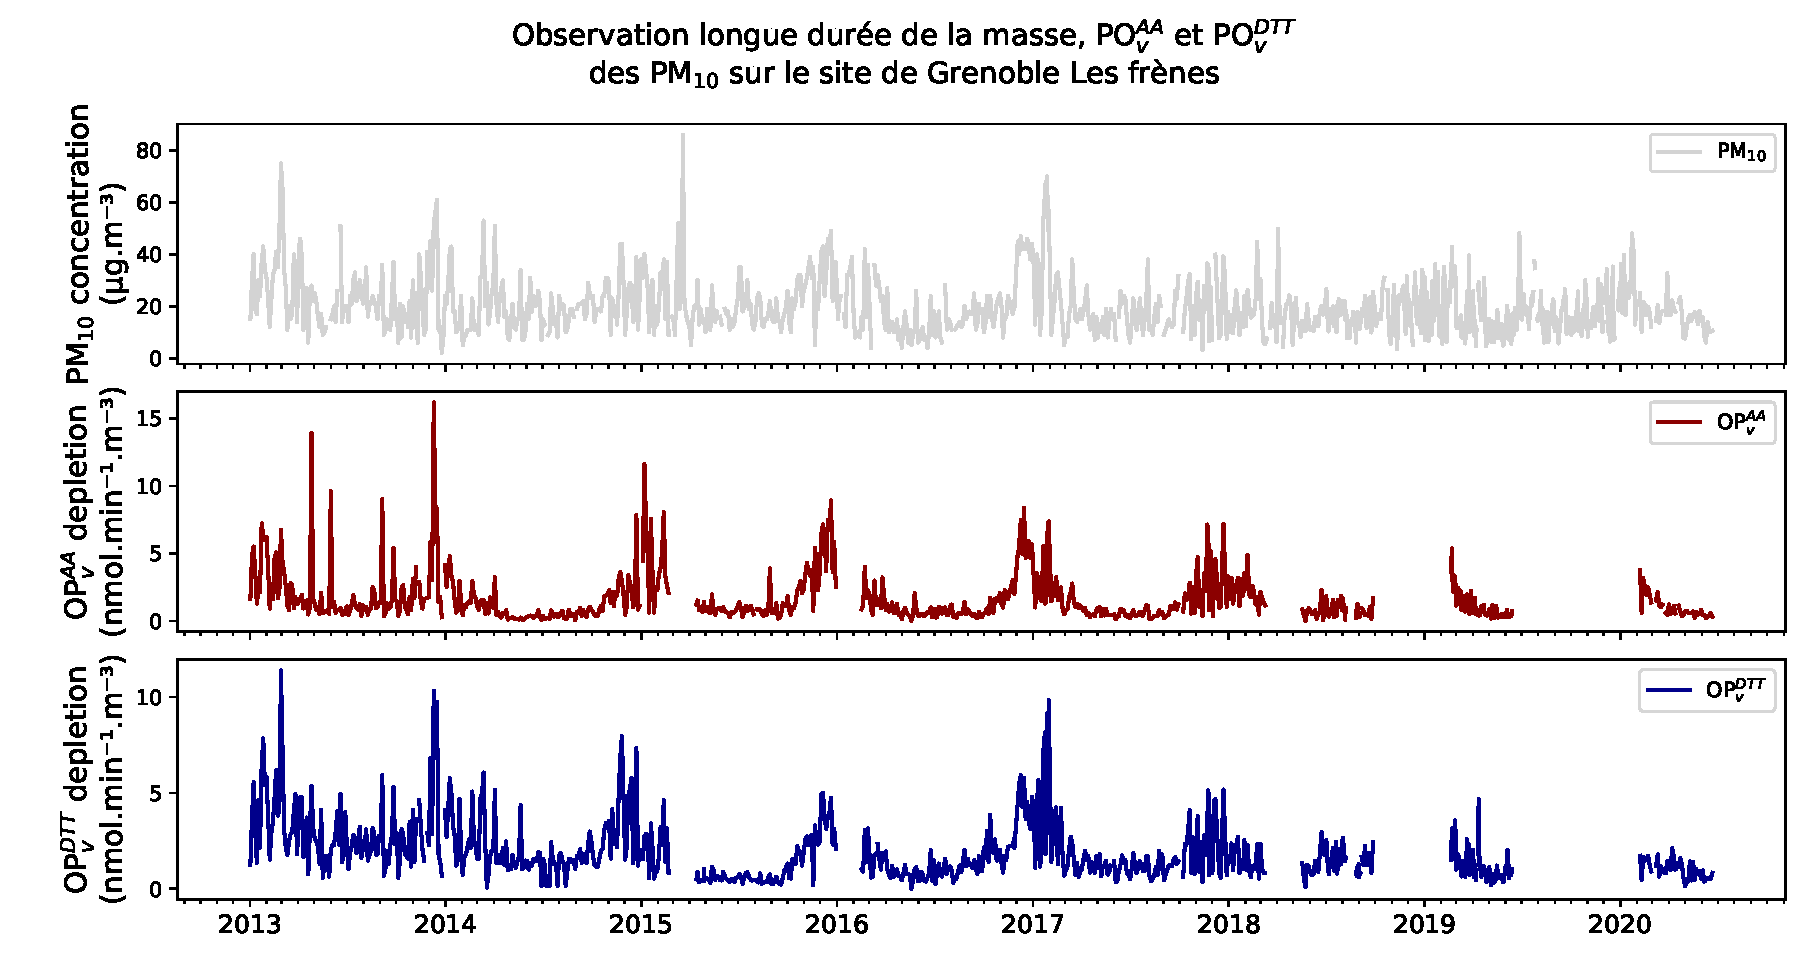
\includegraphics[width=1.0\linewidth]{figures/chapter04/frenes.pdf}
    \caption{Mesure d'observation de la masse des \PMdix, du \POAA{} et du \PODTT{} sur le
    site de Grenoble Les Frènes (GRE-fr) depuis 2013. La masse des \PMdix{} provient des
mesures quotidiennes d'Atmo AURA.}%
\label{fig:TSGREfr}
\end{figure}

\begin{table}[ht]
    \centering
    \caption{Statistiques descriptives et évolution annuelle du \POAAv, \PODTTv{} et masse
    des \PMdix{} sur le site de Grenoble Les Frènes depuis 2013.\\
    Attention, ce travail est encore en cours et la fréquence d'échantillonage varie selon
    les années (voir figure~\ref{fig:TSGREfr}). Notamment, le PO pour 2018 et 2019 ne
    couvre pas une année complète.
}
    \label{tab:statGREfr}
    \sisetup{separate-uncertainty=false}
    \footnotesize
    \begin{tabular}{cccSSSSSSSS}
        \toprule
        variable               & {year} & {count} & {mean}                          & {std} & {min} & {25\%} & {50\%} & {75\%} & {max}\\ \midrule
                               &        &         & \multicolumn{7}{c}{\si{\opv}}\\
\multirow{8}{*}{OP$^{{AA}}_v$} & 2013   & 119     & 2.324                           & 2.606 & 0.257 & 0.904  & 1.385  & 2.553  & 16.185\\
                               & 2014   & 121     & 1.093                           & 1.151 & 0.040 & 0.345  & 0.753  & 1.441  & 7.839\\
                               & 2015   & 103     & 2.269                           & 2.292 & 0.164 & 0.718  & 1.109  & 3.450  & 11.652\\
                               & 2016   & 107     & 1.484                           & 1.638 & 0     & 0.506  & 0.905  & 1.673  & 8.369\\
                               & 2017   & 120     & 1.624                           & 1.726 & 0.119 & 0.469  & 0.941  & 1.974  & 7.372\\
                               & 2018   & 92      & 1.131                           & 0.864 & 0.003 & 0.513  & 0.913  & 1.549  & 4.905\\
                               & 2019   & 107     & 1.124                           & 0.982 & 0.150 & 0.447  & 0.758  & 1.420  & 5.366\\
                               & 2020   & 42      & 0.993                           & 0.819 & 0.188 & 0.463  & 0.671  & 1.187  & 3.796\\\midrule
                               &        &         & \multicolumn{7}{c}{\si{\opv}}\\
\multirow{8}{*}{OP$^{{DTT}}_v$}& 2013   & 119     & 3.081                           & 1.983 & 0.564 & 1.771  & 2.643  & 3.819  & 11.402\\
                               & 2014   & 121     & 2.219                           & 1.566 & 0.059 & 1.320  & 1.694  & 2.473  & 7.965\\
                               & 2015   & 103     & 1.367                           & 1.230 & 0.170 & 0.446  & 0.810  & 2.243  & 5.002\\
                               & 2016   & 107     & 1.609                           & 1.248 & 0     & 0.765  & 1.236  & 2.006  & 5.931\\
                               & 2017   & 120     & 2.034                           & 1.859 & 0.335 & 0.893  & 1.374  & 2.365  & 9.855\\
                               & 2018   & 92      & 1.436                           & 0.611 & 0.072 & 0.931  & 1.354  & 1.840  & 2.938\\
                               & 2019   & 107     & 1.176                           & 0.772 & 0.173 & 0.637  & 1.015  & 1.407  & 4.679\\
                               & 2020   & 42      & 1.000                           & 0.493 & 0.136 & 0.543  & 0.955  & 1.419  & 2.109\\ \midrule
                               &        &         & \multicolumn{7}{c}{\si{\ugm}}\\
\multirow{8}{*}{PM$_{{10}}$}   & 2013   & 351     & 24.38                           & 13.73 & 2     & 14.5   & 22     & 30     & 83\\
                               & 2014   & 360     & 20.38                           & 10.13 & 4     & 13     & 19     & 25     & 67\\
                               & 2015   & 357     & 22.81                           & 11.15 & 4     & 14     & 20     & 29     & 86\\
                               & 2016   & 352     & 19.03                           & 11.50 & 3     & 11     & 16     & 24     & 57\\
                               & 2017   & 350     & 19.62                           & 11.37 & 3     & 12     & 17     & 24     & 70\\
                               & 2018   & 366     & 17.21                           & 7.62  & 3.1   & 12.12  & 16.15  & 21.7   & 49.8\\
                               & 2019   & 352     & 17.21                           & 7.90  & 4.6   & 11.2   & 15.6   & 22.02  & 48.2\\
                               & 2020   & 190     & 17.91                           & 8.25  & 5.2   & 12.65  & 16.8   & 21.12  & 54.3\\
        \bottomrule
    \end{tabular}
\end{table}


\subsection{Variation du PO selon la fraction prélevée (\PMdix{} ou \PMdc)}%
\label{sub:pm10_pm2_5}

Les différentes tailles des particules ne pénétrant pas de façon identique dans le système
respiratoire, la variation du \POv{} par classe de taille est une information importante
pour de futures études épidémiologiques~\cite{fangOxidative2019}.

Sur 6 sites de suivi de la qualité de l'air en Suisse opérés par l'EMPA, les prélèvements conjoints de la fraction grossière
\PMdix{} et plus fine \PMdc{} ont été analysés en PO et sont présentés pour le site de
Berne figure~\ref{fig:PO_berne} pour juin 2018 à mai 2019. La saisonnalité observée sur
les sites français est bien retrouvée pour les \POv{} des \PMdix, et dans une moindre
mesure pour les \POv{} des \PMdc.

En plus de la distribution des valeurs de \POv{} figure~\ref{fig:PO_berne}, la
figure~\ref{fig:PO_berne_ratio_PM10_PM25} présente les ratios \POv{} \PMdc/\PMdix{} pour
l'année complète. 
Premièrement, on constate que les \POv{} des \PMdix{} sont toujours supérieurs aux \POv{}
des \PMdc, ce qui s'explique du fait que les \PMdc{} sont incluses dans la fraction
\PMdix. Plus exactement, le \POv{} des \PMdc{} est en moyenne 2.5 fois plus bas que le
\POv{} des \PMdix{} pour chacun des PO. Ce résultat conforte l'influence des métaux de
transition comme le cuivre sur le PO des PM, ces derniers se retrouvant majoritairement
dans la fraction grossière des PM \todo{(range moyen des non-exhaust emissions ~4µm,  ref de Roy Harrison)}.
En revanche, ces ratios sont variables selon la saison. En effet, les \POAAv{} sont
plus proche en hiver (ratio \PMdc/\PMdix{} = \num{0.62(9)} en janvier) qu'en été (ratio
\PMdc/\PMdix{} = \num{0.25(5)} en juillet). Cette tendance semble plus faible pour le
\PODTTv, notamment du fait de faible valeur de \PODTTv{} des \PMdix{} en juillet et août
2018, induisant un ratio élevé du \PODTTv{} \PMdc/\PMdix{} sur cette période.
On retrouve ici les résultats de \cite{perronePM22019}, sur les mêmes fractions de taille 
mais sur un site méditerranéen. De même, \cite{paraskevopoulouYearlong2019} montre un PO 
différent pour la fraction fine \SI{<2.5}{nm} et celle comprise entre \SIrange{2.5}{10}{nm},
avec également une importance plus grande de la faction fine en hiver.

Cette tendance à des ratios plus élevés en période froide qu'en période chaude renforce
l'hypothèse de l'importance de la source ``combustion de biomasse'' , car les HULIS et
quinones émises par cette source se retrouvent principalement dans la fraction fine
\PMdc{}\autocite{linAbundance2010,fangOxidative2019} et sont connus pour avoir un impact
important sur le PO~\autocite{vermaFractionating2015,maSources2018} et affecteront donc à
la fois les \POv{} des \PMdc{} et \PMdix.

Afin de poursuivre cette investigation, une étude comparative sur 6 sites suisses est
en court à l'EMPA (PI Christoph Huglin, Post-doc Stuart Grange) et à laquelle je prends part, sur les fractions \PMdix{} et
\PMdc. Chacune de ces fractions est analysée pour les tests de \POAA{} et \PODTT{} mais également en
chimie détaillée, permettant à terme une comparaison chimie-PO, et même PMF-PO, selon la
fraction fine et grossière des particules.

\begin{figure}[ht]
    \centering
    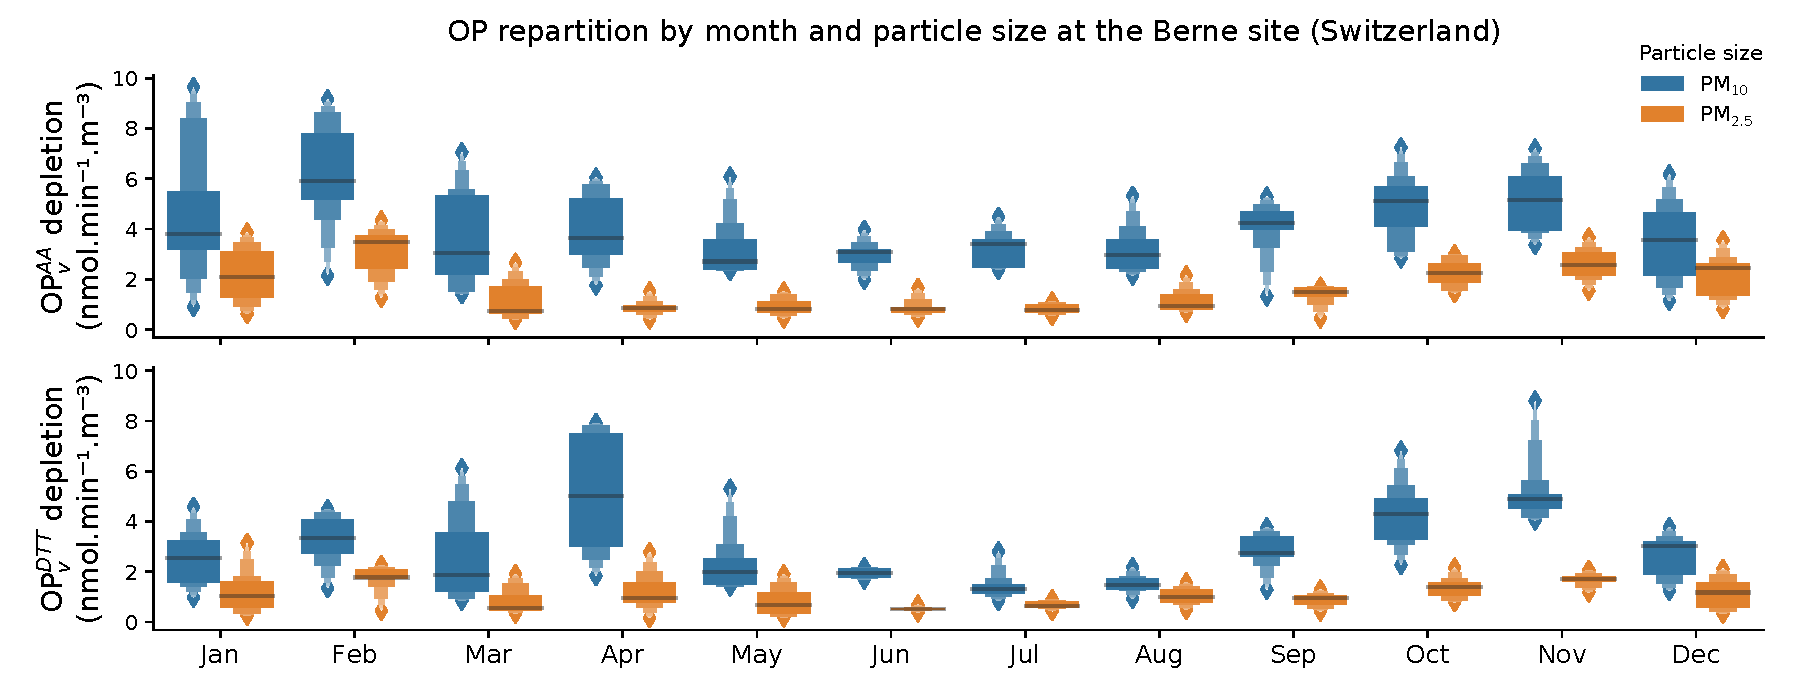
\includegraphics[width=1.0\linewidth]{figures/chapter04/PO_berne.pdf}
    \caption{Variation mensuelle du \POAAv{} et \PODTTv{} sur le site de Berne (Suisse)
    pour la fraction \PMdix{} et \PMdc{} (juin 2018 à mai 2019).}%
    \label{fig:PO_berne}
\end{figure}

\begin{figure}[ht]
    \centering
    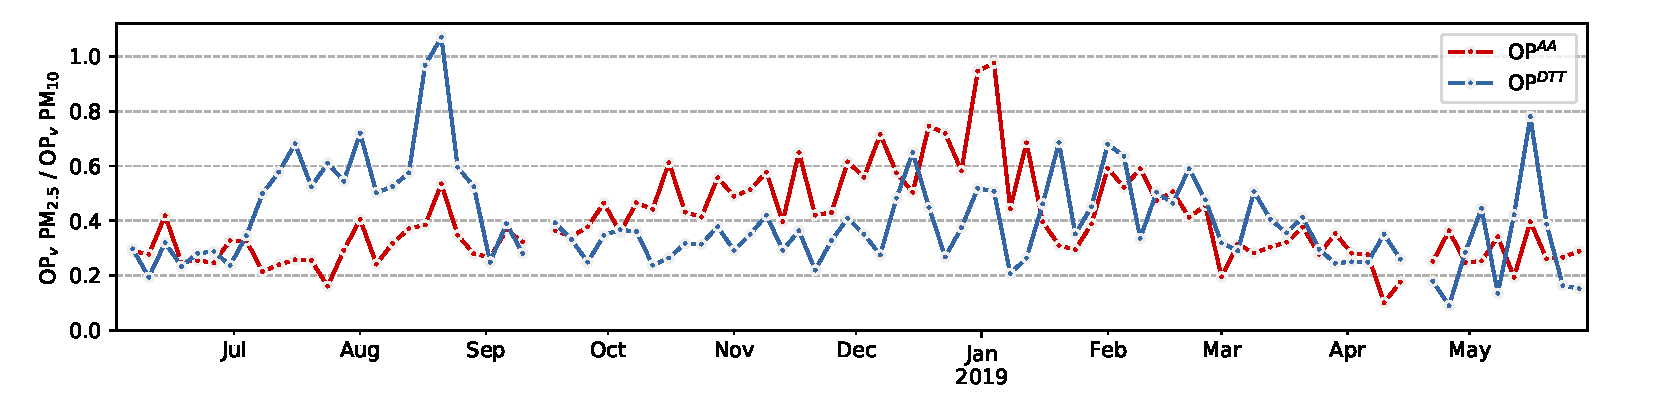
\includegraphics[width=1\linewidth]{figures/chapter04/PO_berne_ratio_PM10_PM25.pdf}
    \caption{Évolution temporelle du ratio \POAAv{} et \PODTTv{} des \PMdix{} sur \POAAv{}
    et \PODTTv{} des \PMdc{} sur le site de Berne.}%
    \label{fig:PO_berne_ratio_PM10_PM25}
\end{figure}

\todo{Tu en étais là Gaëlle, j'ai accepté avant.}


\clearpage
\section{Développement méthodologique à Chamonix}%
\label{ssub:développement_méthodologique_à_chamonix}

\subsection{Le PO par sources d'émission}%
\label{sub:le_po_par_sources_d_émission}

Comme expliqué précédemment, la connaissance des ROS émis ou induits par les PM de
chacune des sources d'émissions majeures permettrait la mise en place de mesure de
protection de la qualité de l'air plus efficace qu'une régulation fondée uniquement sur la
masse des particules.
Cette mesure des ROS peut être estimée en premier ordre par la mesure du PO des PM.
Seulement, certaines catégories de PM ne pourront tout simplement pas être directement
mesurées aux PO, ou nécessiteraient des conditions très opportunistes (formation de nitrate
d'ammonium secondaire, fort épisode de vent saharien, émission biogénique primaire, etc.).

Afin de néanmoins prendre en compte ces processus, il a été choisi de conduire des études
sur site à l'aide du modèle source-recepteur PMF. Sur chacun des filtres où les espèces
chimiques ont été analysées, le \POv{} a également été mesuré par AA et DTT. Ainsi, suivant
la procédure décrite en figure~\ref{fig:workflow_inversion}, il est possible d'estimer les
source de PM au niveau du site récepteur et de leur attribuer un PO intrinsèque (i.e. par
microgramme de PM), et donc de déterminer la contribution de chacune des sources de PM aux
potentiels oxydants.

La section suivante applique cette méthodologie sur le site expérimental de Chamonix,
France.

\subsection{An apportionment method for the oxidative potential of atmospheric particulate
matter sources: application to a one-year study in Chamonix, France}
\label{sec:weber_et_al_2018}

\begin{tcolorbox}[colback=red!5!white,colframe=Melon,title=Note]
Article paru dans le journal \textit{Atmospheric Chemistry and Physics} le 4 juin 2019 :

\begin{quote}
    Samuël Weber, Gaëlle Uzu, Aude Calas, Florie Chevrier, Jean-Luc Besombes,
    Aurélie Charron, Dalia Salameh, Irena Ježek, Griša Močnik, et Jean-Luc Jaffrezo. 2018.
    \textit{An Apportionment Method for the Oxidative Potential of Atmospheric Particulate
    Matter Sources: Application to a One-Year Study in Chamonix, France}. Atmospheric
    Chemistry and Physics 18(13), pp. 9617‑9629.
    \textsc{doi} : \href{https://doi.org/10.5194/acp-18-9617-2018}{10.5194/acp-18-9617-2018},
    \textsc{url} : \url{https://www.atmos-chem-phys.net/18/9617/2018/}
\end{quote}

Les profils PMF, la corrélation entre espèces chimiques et PO et sources et
PO à titre de comparaison avec les études antérieures, sont présentés en complément de
l'article, repris en annexe~\ref{annexe:deconvol_OP_SI}.
\end{tcolorbox}

\clearpage
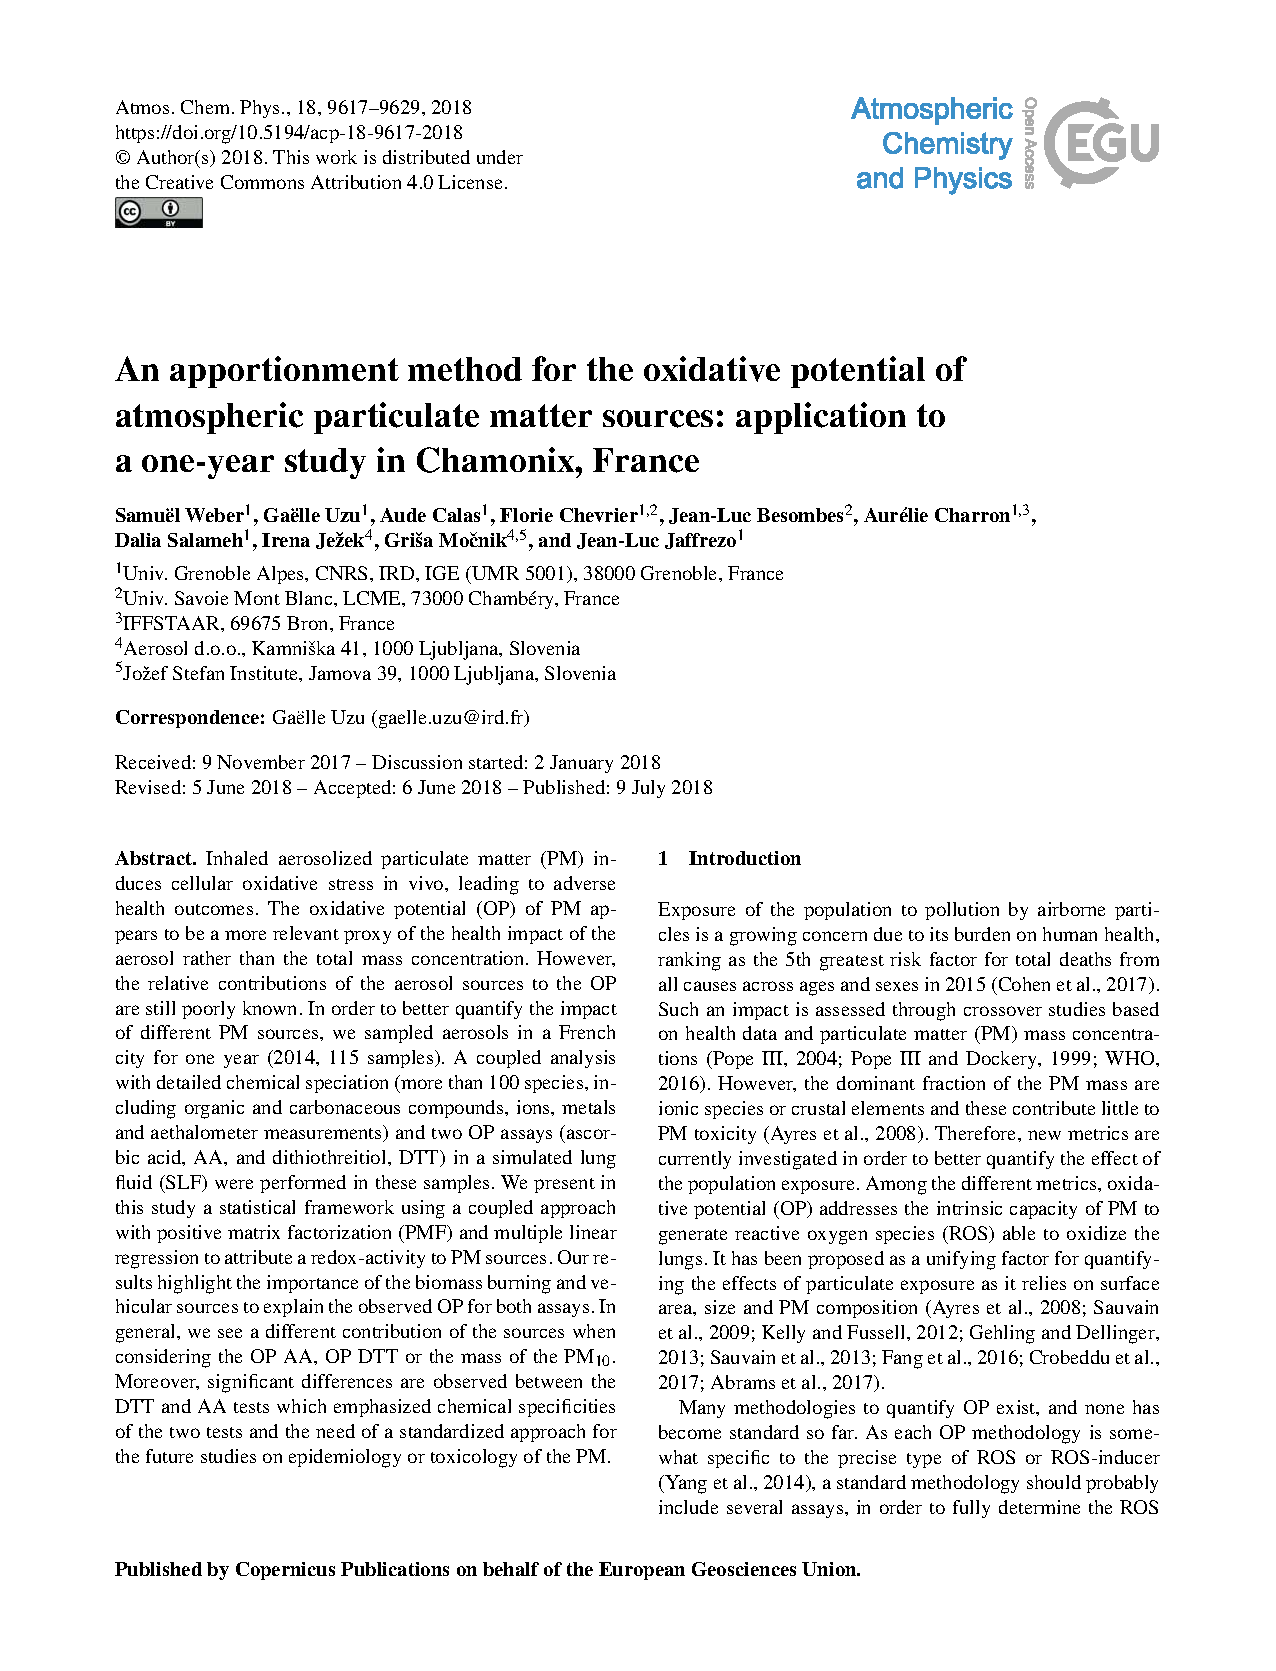
\includepdf[pages=-,scale=0.95,pagecommand={\pagestyle{fancy}}]{chapters/deconvol_OP.pdf}

\subsection{Conclusion}

Cette section prouve tout d'abord qu'il est possible de déterminer les sources de PO grâce à
une étude couplée entre une PMF avancée utilisant différents traceurs organiques résultant
en 8 facteurs distincts et une régression linéaire multiple prenant en compte
la mesure du PO à iso-masse utilisant des conditions de bioaccessibilité proche du milieu
pulmonaire et ses incertitudes, avec une très bonne performance statistique.

Cette méthode permet de différencier très nettement les sources de PM contribuant aux PO
et apporte une vue nouvelle de l'aérosol en redistribuant l'importance de la contribution
des sources. Conformément aux résultats des 3 études précédentes faites aux États-Unis
\autocite{vermaReactive2014,batesReactive2015,fangOxidative2016}, la combustion de
biomasse domestique et le transport routier représentent les 2 sources principales de
\POAAv{} et \PODTTv.

L'utilisation de deux tests de PO nous permet aussi d'affirmer que ces 2 tests ne portent
pas en eux exactement les mêmes informations géochimiques, car les sources de PM les
expliquant diffèrent --bien que la même tendance générale est observée. En l'absence
d'étude approfondie quant aux liens toxicologie-PO ou épidémiologie-PO, le maintient de
différents tests de PO est donc recommandé.

Aussi, certaines corrélations observées, aussi bien avec des espèces chimiques que des
facteurs PMF, s'avère comme attendue trompeuse. Le facteur nitrate-rich était corrélé au
\POAAv{} mais présent en réalité un PO intrinsèque quasi-nul. Inversement, le facteur
secondaire biogénique, tracé par le MSA, est négativement corrélé aux deux \OPv{} alors
qu'il présente le 2\ieme{} \PODTT{} intrinsèque le plus élevé. Il est donc nécessaire
d'utiliser des méthodes statistiques plus avancées que la régression uni-variée lorsque
l'on cherche à estimer les sources de PO afin de s'affranchir des tendances saisonnières et
des covariations entre espèces.

Cette méthode est donc validée comme outil de déconvolution des sources de PO, et le
prochain chapitre traitera de son application à un large panel d'environnement et année
d'étude, afin d'établir à la manière du chapitre précédent, une phénoménologie non pas des
sources de la masse \PMdix, mais des sources de potentiels oxydants de particules.


\section{Pertinence géochimique à grande échelle des sources de PO}%
\label{sec:synthèse_grande_échelle}

\subsection{Introduction}%
\label{sub:introduction_synthèse_nationale}

La méthode de déconvolution des sources de PO établie dans la section précédente permet donc
d'estimer efficacement les PO intrinsèques des différentes sources de PM déterminées par
PMF, avec de meilleures performances statistiques que les études similaires précédentes.
Cela tient probablement au fait de la meilleure prise en compte des différentes sources de
PM grâce à une PMF plus détaillée que celles des études antérieurs et non
perturbée par l'ajout des PO dans le système d'équation de la PMF.

La question suivante est donc naturellement la généralisation ou non de ce résultat.
Est-il possible d'estimer correctement un PO intrinsèque pour chacune des sources de PM
estimée par PMF, indépendamment du lieu de prélèvement ? Si oui, est-ce que chaque source
de PM présente un PO intrinsèque similaire de site en site, et avec quelle variabilité ?

Pour répondre à cette question, un ensemble de 14 sites de prélèvement a minima annuel, couvrant les
années 2013 à 2018 et différents types d'environnements (urbain, trafic, industriel et vallée alpine),
a été choisi pour estimer de manière standardisée leurs sources de PM grâce à la
méthodologie développée dans le cadre du programme SOURCES présentée
section~\ref{sub:article_SOURCES}~\autocite{weberSources2019}. En effet, la PMF présentée précédemment sur le site de
Chamonix n'est pas facilement généralisable, car les espèces chimiques utilisées ne sont
pas disponibles pour un grand nombre de site (hopanes, methoxyphénol et mesure de
l'aethalometre notamment).

Ainsi, les sites du programme SOURCES sur lesquels suffisamment de filtres étaient
disponibles ont été analysées en \POAA{} et \PODTT. Afin d'enrichir et améliorer la
représentativité spatiale de l'étude, j'ai également pris en compte de nouvelles études
PMF, similaires à la méthodologie SOURCES, faite spécifiquement dans le cadre de cette
étude, pour les sites de Passy, Marnaz, GRE-fr (2017), GRE-cb, et Vif.
Aussi, le site de Rouen présentant un résultat PMF indiquant de potentiels mélanges de
facteurs a été écarté de cette étude \autocite{weberComparison2019}.

C'est donc plus de 1700 filtres répartis sur 14 sites de prélèvements et 15 séries
annuelles complètes (voir tableau 1 de l'article suivant) analysées analytiquement suivant
un protocol standard à tous les échantillons et statistiquement par des PMF harmonisées
qui permettront, ou non, la généralisation de cette méthode de déconvolution des sources
de PO.

\begin{tcolorbox}[colback=red!5!white,colframe=Melon,title=Note]
    Devant la quantité de résultat à présenter (résultat PMF, similitude géochimique des
    facteurs entre sites, séries temporelles des PO, performance statistiques,
    contribution saisonnières des sources aux PO, etc.), le choix a été pris de rendre
    disponible l'ensemble des données et de facilité leur visualisation à travers le site
    \url{http://getopstandop.u-ga.fr}.
    Les résultats agrégés sont présentés dans l'article suivant, mais le détail de chacun
    des sites et facteur PMF peut être retrouvé sur le site.
\end{tcolorbox}

\subsection{Source apportionment of the oxidative potential of aerosols at 15 French
sites for yearly time series of observation}%
\label{sub:article}

\begin{tcolorbox}[colback=red!5!white,colframe=Melon,title=Note]
Article actuellement en préparation pour \textit{Atmospheric Chemistry and Physics} :
\begin{quote}
    Samuël Weber, Gaëlle Uzu, Aude Calas, Dalia Salameh, Florie Chevrier, Julie Allard,
    Jean-Luc Besombes, Olivier Favez, (Les représentants des différentes AASQA), et
    Jean-Luc Jaffrezo. in prep.
    \textit{Source apportionment of the oxidative potential of aerosols at 15 French
    sites for yearly time series of observation}.
\end{quote}
\end{tcolorbox}

\clearpage
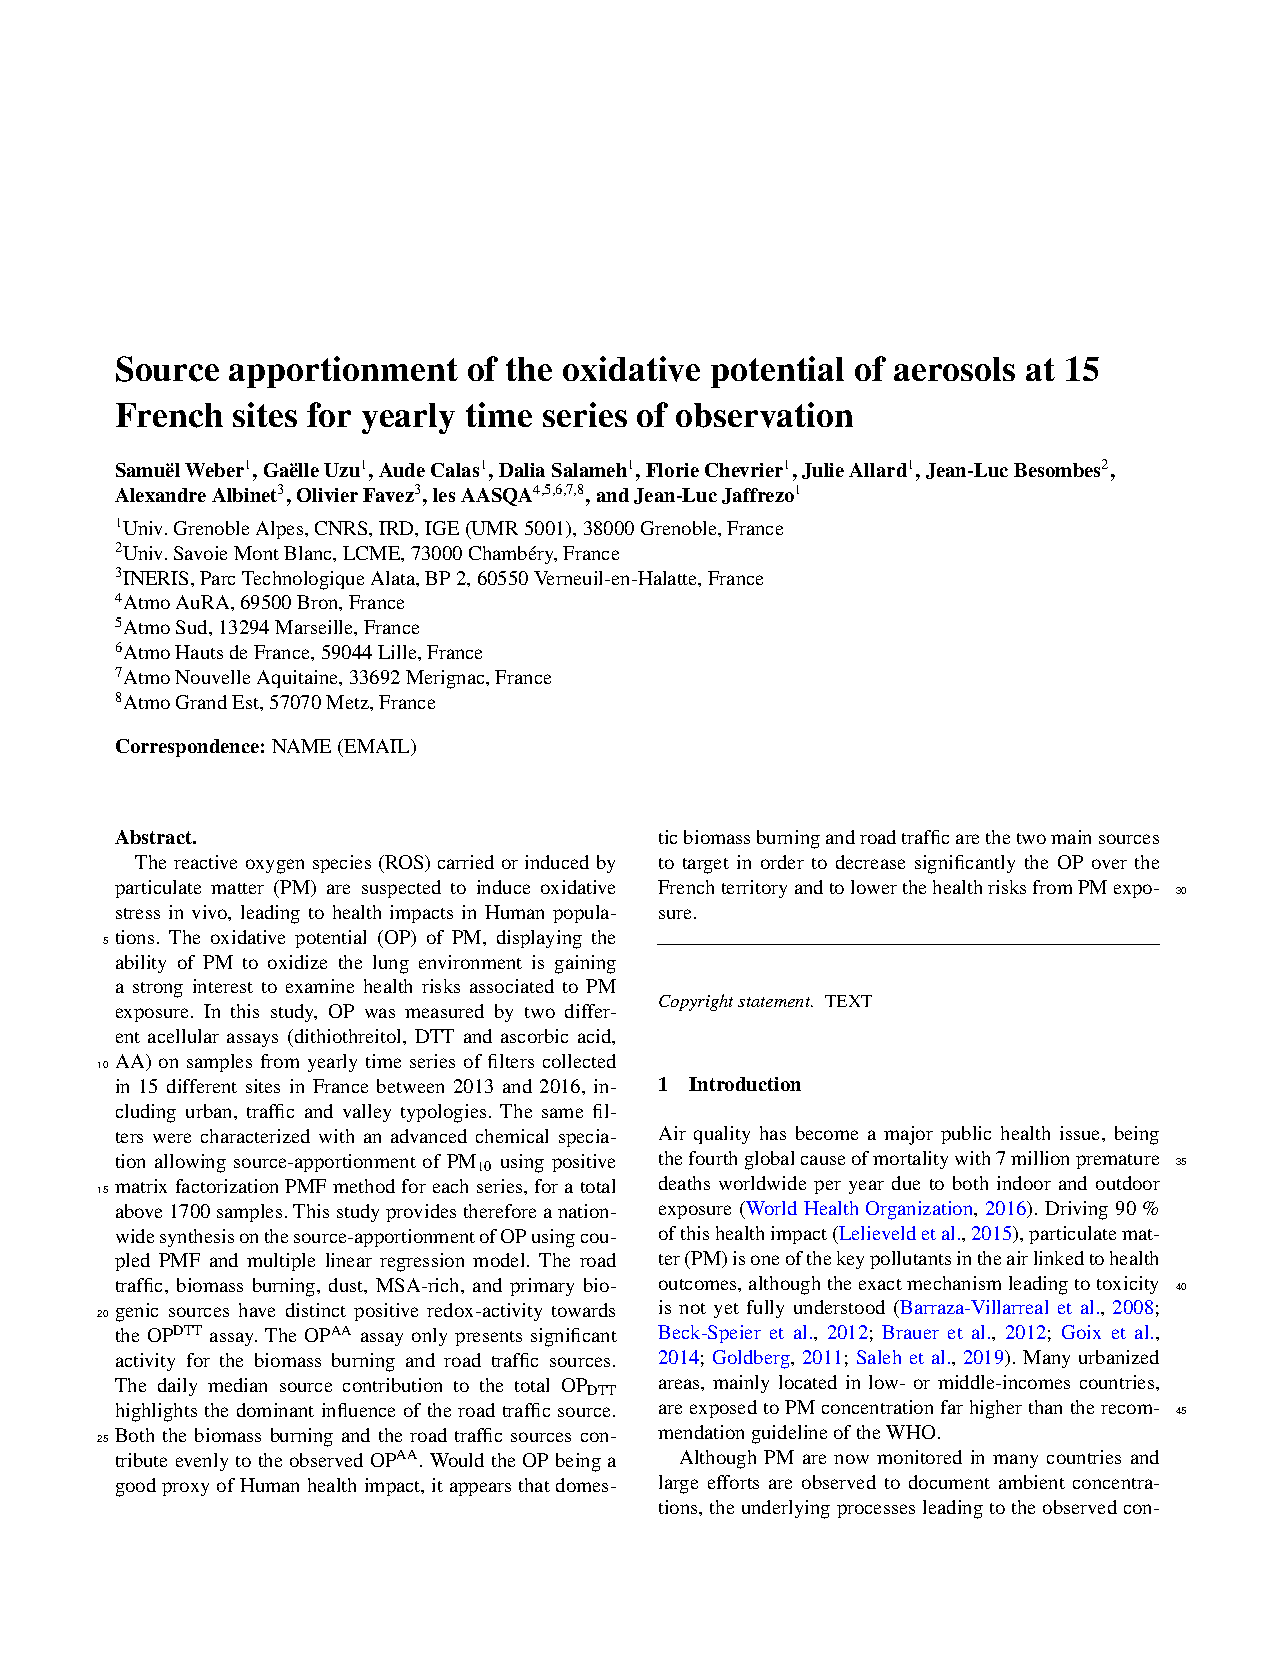
\includepdf[pages=-,scale=0.95,pagecommand={\pagestyle{fancy}}]{chapters/article_allOP/article_nuage.pdf}

\subsection{Conclusion}%
\label{sec:conclusion_synthèse_OP}

\subsubsection{Une méthodologie statistiquement et géochimiquement validée}%
\label{ssub:une_méthodologie_statistiquement_et_géochimiquement_validée}

La méthode d'estimation des sources de \POAA{} et \PODTT{} des \PMdix{} couplant des
analyses PMF avancées et un modèle d'inversion linéaire prenant en compte les incertitudes
des mesures de PO présente des résultats statistiques très satisfaisant pour l'ensemble
des sites étudiés ($r^2>0.7$ et intercept faible, à l'exception notable de VIF (\PODTT) et
STG-cle (\POAA)).

Les mêmes sources de \PMdix{} déterminées grâces à des PMF harmonisées présentes un potentiel
oxydant intrinsèque (i.e. par microgramme de PM) similaire, et ce, pour différents types
d'environnements (urbain, industriel, trafic et vallée alpine). Une étude à si large
échelle spatiale et temporelle, utilisant à la fois le \POAA{} et \PODTT{} nous permet
donc de conclure que les PO sont bien distincts selon la source --et donc la géochimie--
considérés, et chaque type de source présent un PO intrinsèque déterminé et indépendant du
site d'étude.

Ce résultat était un préalable nécessaire à la modélisation du PO par les modèles
déterministes CTM afin d'établir une couverture spatiale et temporelle beaucoup plus
large que les études sur sites, permettant à terme des études épidémiologiques sur la
qualité de l'air à travers la métrique du potentiel oxydant.

\subsubsection{Une redistribution de l'importance des sources de PM}%
\label{ssub:une_redistribution_de_l_importance_des_sources_de_pm}

Sans attendre la modélisation CTM, il est d'ors et déjà possible de dire que les
différentes sources de PM présentes des PO intrinsèques distincts et qu'il y a une
redistribution complète de l'importance de la contribution des sources aux \PMdix{} selon
la métrique d'observation choisi : masse, \POAAv{} ou \PODTTv. Les sources inorganiques
secondaires (nitrate-rich et sulfate-rich) contribuant significativement à la masse de PM
ne contribuent en définitive que peu aux PO. Ainsi, sous l'hypothèse que
la métrique du PO permet une meilleure estimation de la toxicité des PM, les sources
d'émissions d'importances sanitaires présentes sur l'ensemble de la France se trouvent être
principalement 2 sources d'émissions primaires anthropiques : le trafic routier et la
combustion de biomasse domestique. Ces résultats concordent avec les études précédentes de
\cite{batesReactive2015,fangOxidative2016}, et celles plus récentes de
\cite{paraskevopoulouYearlong2019,cesariSource2019}. Il est également intéressant de
voir que l'étude de \cite{cesariSource2019} a confronté les approches 2 approches ``PO comme variable
dans la PMF'' ou ``PO estimé par régression linéaire des résultats PMF'', et lors
de l'ajout du \PODTTv{} dans la PMF, la source traffic se voit attribuer davantage de Fe
et Cr et beaucoup moins de nitrate et ammonium.

Il est à noter que ces 2 sources ont cependant des dynamiques très différentes. L'émission
primaire du trafic présente un fort PO intrinsèque pour les deux tests de PO.
En revanche, si la combustion de biomasse domestique présente un \POAA{} intrinsèque du
même ordre que le trafic routier, son \PODTT{} intrinsèque est près de 2 fois plus
faible. Aussi, l'importance de la combustion de biomasse vient principalement du fait des
fortes concentrations de cette source durant l'hiver. L'exposition à cette source est donc
importante en hiver mais absente en dehors de cette saison à l'inverse de l'émission
primaire du trafic présentant de plus faibles concentrations mais tout au long de l'année.
Selon l'importance d'une exposition aigüe ou chronique aux PO, il conviendra donc de
cibler d'abord l'une ou l'autre de ces sources.

Parmi les sources naturelles, les émissions primaires biogéniques et les poussières
crustales présentes également une activité rédox importante pour le test au \PODTT, mais
pas pour le \POAA, retrouvant ainsi en condition ambiante les résultats de mesure de PO
sur les bioaérosols de \cite{samakeUnexpected2017}.

Cependant, les processus secondaires semblent également pouvoir jouer un rôle important
dans le PO ambiant, mais l'incertitude liée à cette source est trop grande pour en tirer
des conclusions avec les connaissances dont nous disposons actuellement. Cette
incertitude est très certainement liée à la difficulté de la prise en compte des sources
ou processus conduisant à la formation d'aérosols organiques secondaires par les PMF avec
spéciation chimique sur filtres.
\todo{une figure avec PO avec acide orga ?}


\section{Conclusion du chapitre}%
\label{sec:conclusion_chap4}

\subsection{Une nouvelle vision de l'aérosol, plus proche de l'impact sanitaire}%
\label{sub:une_nouvelle_vision_de_l_aérosol_plus_proche_de_l_impact_sanitaire}

Grâce à la mise en place et l'harmonisation des nombreuses mesures de chimie et de PO
ainsi que des résultats issus PMF au sein d'une base de donnée unique, il a été possible
d'établir une phénoménologie des sources de \POAA{} et \PODTT{} à grande échelle spatiale.

Au cours des dernières années, cette base de donnée s'est considérablement enrichie et
d'autres groupes de recherches ont commencé à documenter à large échelle spatiale des
résultats similaires en Italie~\autocite{pietrograndeReview2019} ou en
Suisse\footnote{Mesures effectuées par l'IGE} grâce au
PSI~\autocite{daellenbachSourcessubmitted} ou l'EMPA et des travaux sont également en
cours pour une collaboration avec le TNO au Pays-bas et l'IDAEA en Espagne dans le cadre
de l'ANR GetOP-StandOP portée par Gaëlle Uzu.
\todo{est-ce qu'on peut dire ca?}

À travers ces travaux et l'établissement de méthode de déconvolution des sources de PO, il
est montré que la vision que l'on a de l'aérosol à travers la métrique de la
concentration massique doit être repensé lorsque l'on s'intéresse à l'impact sanitaire
des sources de PM. Les sources contribuants majoritairement à la masse des PM n'étant pas
nécessairement celles contribuant le plus aux \POAA{} ou \PODTT, et inversement.
Ainsi, au cours des dernières années, les études aux \POAA{} et \PODTT{} de
\cite{vermaReactive2014,batesReactive2015,fangOxidative2016,weberApportionment2018,cesariSource2019,daellenbachSourcessubmitted,weberSourceinprep.}
semblent indiquer la prédominance de 2 sources anthropiques majoritaire pour l'exposition
aux PO : le traffic routier et la combustion de biomasse domestique.

En revanche, concernant l'exposition chronique, nous avons montré qu'il est clair que
l'émission primaire du trafic routier est la source majoritaire du potentiel oxydant des
aérosols, aussi bien au \POAA{} qu'au \PODTT. Ce secteur d'émission est dans notre étude
la seule source ayant un impact très important aussi bien sur la concentration médiane des
\PMdix{}, le \POAAv{} et le \PODTTv.
Ainsi, même si la ``meilleure'' métrique de l'impact sanitaire n'est pas définitivement
connu à ce jour, ces 3 métriques convergent vers l'importance du trafic routier. Ce
résultat, intuitif car il est connu empiriquement depuis longtemps qu'il vaut mieux ne
pas respirer derrière un pot d'échappement, est néanmoins encourageant, car de nombreuses
villes et métropole, mais aussi individus, se dirigent d'ors et déjà vers une diminution
de l'utilisation de la voiture individuelle. Il est donc espérable d'avoir dans les années
futures à la fois une lutte efficace contre le dérèglement climatique et une amélioration
de la qualité de l'air.

\subsection{Limitation et travaux futur}%
\label{sub:limitation_et_travaux_futur}

Bien que présentant certaines avancées importantes, les travaux de cette thèse présentes
des limitations à prendre en compte.

Tout d'abord, la méthodologie de déconvolution des sources de PO des PM utilise un modèle
linéaire. Or, le PO, et notamment le \PODTT, est connu pour ne pas réagir de manière
linéaire avec la masse des espèces
chimiques~\autocite{charrierDithiothreitol2012,sauvainComparison2013,charrierRates2015,charrierBias2016,calasImportance2017}.
Aussi, aucun
terme d'interaction entre les sources n'est pris en compte dans ces modèles, or il est
envisageable que, par exemple, un aérosol sulfaté et donc plus acide augmente la
solubilisation des particules et donc présente un PO différent du fait uniquement de la
présence de sulfate.  La prise en compte de ces non-linéarités et des actions conjointes
des différentes sources sur les PO serait certainement un ajout important et changerait
potentiellement les résultats présentés ici. Le chapitre suivant explore l'une des façons
possibles d'estimer l'importance de cette non linéarité à partir d'un réseau de neurone.

La variation infra-journalière du PO est également encore peu documenté, et uniquement
pour la mesure du PO par DCFH \autocite{venkatachariMeasurement2005,costabileFirst2017}.
Cependant, plusieurs travaux vont en ce sens
\autocite{zhouDevelopment2018,jovanovicMeasurements2019} et montrent la forte variation
journalière des potentiels oxydants.  La moyenne journalière utilisée jusqu'à présent est
donc un premier pas, mais il apparaît nécessaire d'obtenir une résolution temporelle plus
fine.  Des développements méthodologiques pour coupler les différentes mesures hautes
fréquences possible (AMS, aethalometre, XRF, and ROS online) afin de déterminer la raison
de cette variabilité.

Finalement, et en lien avec le paragraphe précédent, il est également nécessaire pour
comprendre les liaisons entre potentiel oxydant et impacte sanitaire d'augmenter la
couverture spatiale de mesure ou d'estimation des PO. L'outil le plus adapté pour cela est
la modélisation déterministe à travers les modèles CTM, permettant la prédiction et la
ré-analyse spatiale et temporelle du potentiel oxydant des aérosols. Maintenant que nous
avons montré que le PO intrinsèque des différentes sources est stable géographiquement,
il est envisageable d'estimer géographiquement les PO à partir de ces modèles. Deux
exemples en cours sont présentés dans le chapitre suivant.
